
%% bare_conf.tex
%% V1.3
%% 2007/01/11
%% by Michael Shell
%% See:
%% http://www.michaelshell.org/
%% for current contact information.
%%
%% This is a skeleton file demonstrating the use of IEEEtran.cls
%% (requires IEEEtran.cls version 1.7 or later) with an IEEE conference paper.
%%
%% Support sites:
%% http://www.michaelshell.org/tex/ieeetran/
%% http://www.ctan.org/tex-archive/macros/latex/contrib/IEEEtran/
%% and
%% http://www.ieee.org/

%%*************************************************************************
%% Legal Notice:
%% This code is offered as-is without any warranty either expressed or
%% implied; without even the implied warranty of MERCHANTABILITY or
%% FITNESS FOR A PARTICULAR PURPOSE! 
%% User assumes all risk.
%% In no event shall IEEE or any contributor to this code be liable for
%% any damages or losses, including, but not limited to, incidental,
%% consequential, or any other damages, resulting from the use or misuse
%% of any information contained here.
%%
%% All comments are the opinions of their respective authors and are not
%% necessarily endorsed by the IEEE.
%%
%% This work is distributed under the LaTeX Project Public License (LPPL)
%% ( http://www.latex-project.org/ ) version 1.3, and may be freely used,
%% distributed and modified. A copy of the LPPL, version 1.3, is included
%% in the base LaTeX documentation of all distributions of LaTeX released
%% 2003/12/01 or later.
%% Retain all contribution notices and credits.
%% ** Modified files should be clearly indicated as such, including  **
%% ** renaming them and changing author support contact information. **
%%
%% File list of work: IEEEtran.cls, IEEEtran_HOWTO.pdf, bare_adv.tex,
%%                    bare_conf.tex, bare_jrnl.tex, bare_jrnl_compsoc.tex
%%*************************************************************************

% *** Authors should verify (and, if needed, correct) their LaTeX system  ***
% *** with the testflow diagnostic prior to trusting their LaTeX platform ***
% *** with production work. IEEE's font choices can trigger bugs that do  ***
% *** not appear when using other class files.                            ***
% The testflow support page is at:
% http://www.michaelshell.org/tex/testflow/



% Note that the a4paper option is mainly intended so that authors in
% countries using A4 can easily print to A4 and see how their papers will
% look in print - the typesetting of the document will not typically be
% affected with changes in paper size (but the bottom and side margins will).
% Use the testflow package mentioned above to verify correct handling of
% both paper sizes by the user's LaTeX system.
%
% Also note that the "draftcls" or "draftclsnofoot", not "draft", option
% should be used if it is desired that the figures are to be displayed in
% draft mode.
%
\documentclass[conference]{IEEEtran}
\usepackage{blindtext, graphicx, hyperref, amsmath, fixmath, graphicx, caption, amssymb, tabu}
\graphicspath{ {images/} }
% Add the compsoc option for Computer Society conferences.
%
% If IEEEtran.cls has not been installed into the LaTeX system files,
% manually specify the path to it like:
% \documentclass[conference]{../sty/IEEEtran}





% Some very useful LaTeX packages include:
% (uncomment the ones you want to load)


% *** MISC UTILITY PACKAGES ***
%
%\usepackage{ifpdf}
% Heiko Oberdiek's ifpdf.sty is very useful if you need conditional
% compilation based on whether the output is pdf or dvi.
% usage:
% \ifpdf
%   % pdf code
% \else
%   % dvi code
% \fi
% The latest version of ifpdf.sty can be obtained from:
% http://www.ctan.org/tex-archive/macros/latex/contrib/oberdiek/
% Also, note that IEEEtran.cls V1.7 and later provides a builtin
% \ifCLASSINFOpdf conditional that works the same way.
% When switching from latex to pdflatex and vice-versa, the compiler may
% have to be run twice to clear warning/error messages.






% *** CITATION PACKAGES ***
%
%\usepackage{cite}
% cite.sty was written by Donald Arseneau
% V1.6 and later of IEEEtran pre-defines the format of the cite.sty package
% \cite{} output to follow that of IEEE. Loading the cite package will
% result in citation numbers being automatically sorted and properly
% "compressed/ranged". e.g., [1], [9], [2], [7], [5], [6] without using
% cite.sty will become [1], [2], [5]--[7], [9] using cite.sty. cite.sty's
% \cite will automatically add leading space, if needed. Use cite.sty's
% noadjust option (cite.sty V3.8 and later) if you want to turn this off.
% cite.sty is already installed on most LaTeX systems. Be sure and use
% version 4.0 (2003-05-27) and later if using hyperref.sty. cite.sty does
% not currently provide for hyperlinked citations.
% The latest version can be obtained at:
% http://www.ctan.org/tex-archive/macros/latex/contrib/cite/
% The documentation is contained in the cite.sty file itself.






% *** GRAPHICS RELATED PACKAGES ***
%
\ifCLASSINFOpdf
  % \usepackage[pdftex]{graphicx}
  % declare the path(s) where your graphic files are
  % \graphicspath{{../pdf/}{../jpeg/}}
  % and their extensions so you won't have to specify these with
  % every instance of \includegraphics
  % \DeclareGraphicsExtensions{.pdf,.jpeg,.png}
\else
  % or other class option (dvipsone, dvipdf, if not using dvips). graphicx
  % will default to the driver specified in the system graphics.cfg if no
  % driver is specified.
  % \usepackage[dvips]{graphicx}
  % declare the path(s) where your graphic files are
  % \graphicspath{{../eps/}}
  % and their extensions so you won't have to specify these with
  % every instance of \includegraphics
  % \DeclareGraphicsExtensions{.eps}
\fi
% graphicx was written by David Carlisle and Sebastian Rahtz. It is
% required if you want graphics, photos, etc. graphicx.sty is already
% installed on most LaTeX systems. The latest version and documentation can
% be obtained at: 
% http://www.ctan.org/tex-archive/macros/latex/required/graphics/
% Another good source of documentation is "Using Imported Graphics in
% LaTeX2e" by Keith Reckdahl which can be found as epslatex.ps or
% epslatex.pdf at: http://www.ctan.org/tex-archive/info/
%
% latex, and pdflatex in dvi mode, support graphics in encapsulated
% postscript (.eps) format. pdflatex in pdf mode supports graphics
% in .pdf, .jpeg, .png and .mps (metapost) formats. Users should ensure
% that all non-photo figures use a vector format (.eps, .pdf, .mps) and
% not a bitmapped formats (.jpeg, .png). IEEE frowns on bitmapped formats
% which can result in "jaggedy"/blurry rendering of lines and letters as
% well as large increases in file sizes.
%
% You can find documentation about the pdfTeX application at:
% http://www.tug.org/applications/pdftex





% *** MATH PACKAGES ***
%
%\usepackage[cmex10]{amsmath}
% A popular package from the American Mathematical Society that provides
% many useful and powerful commands for dealing with mathematics. If using
% it, be sure to load this package with the cmex10 option to ensure that
% only type 1 fonts will utilized at all point sizes. Without this option,
% it is possible that some math symbols, particularly those within
% footnotes, will be rendered in bitmap form which will result in a
% document that can not be IEEE Xplore compliant!
%
% Also, note that the amsmath package sets \interdisplaylinepenalty to 10000
% thus preventing page breaks from occurring within multiline equations. Use:
%\interdisplaylinepenalty=2500
% after loading amsmath to restore such page breaks as IEEEtran.cls normally
% does. amsmath.sty is already installed on most LaTeX systems. The latest
% version and documentation can be obtained at:
% http://www.ctan.org/tex-archive/macros/latex/required/amslatex/math/





% *** SPECIALIZED LIST PACKAGES ***
%
%\usepackage{algorithmic}
% algorithmic.sty was written by Peter Williams and Rogerio Brito.
% This package provides an algorithmic environment fo describing algorithms.
% You can use the algorithmic environment in-text or within a figure
% environment to provide for a floating algorithm. Do NOT use the algorithm
% floating environment provided by algorithm.sty (by the same authors) or
% algorithm2e.sty (by Christophe Fiorio) as IEEE does not use dedicated
% algorithm float types and packages that provide these will not provide
% correct IEEE style captions. The latest version and documentation of
% algorithmic.sty can be obtained at:
% http://www.ctan.org/tex-archive/macros/latex/contrib/algorithms/
% There is also a support site at:
% http://algorithms.berlios.de/index.html
% Also of interest may be the (relatively newer and more customizable)
% algorithmicx.sty package by Szasz Janos:
% http://www.ctan.org/tex-archive/macros/latex/contrib/algorithmicx/




% *** ALIGNMENT PACKAGES ***
%
%\usepackage{array}
% Frank Mittelbach's and David Carlisle's array.sty patches and improves
% the standard LaTeX2e array and tabular environments to provide better
% appearance and additional user controls. As the default LaTeX2e table
% generation code is lacking to the point of almost being broken with
% respect to the quality of the end results, all users are strongly
% advised to use an enhanced (at the very least that provided by array.sty)
% set of table tools. array.sty is already installed on most systems. The
% latest version and documentation can be obtained at:
% http://www.ctan.org/tex-archive/macros/latex/required/tools/


%\usepackage{mdwmath}
%\usepackage{mdwtab}
% Also highly recommended is Mark Wooding's extremely powerful MDW tools,
% especially mdwmath.sty and mdwtab.sty which are used to format equations
% and tables, respectively. The MDWtools set is already installed on most
% LaTeX systems. The lastest version and documentation is available at:
% http://www.ctan.org/tex-archive/macros/latex/contrib/mdwtools/


% IEEEtran contains the IEEEeqnarray family of commands that can be used to
% generate multiline equations as well as matrices, tables, etc., of high
% quality.


%\usepackage{eqparbox}
% Also of notable interest is Scott Pakin's eqparbox package for creating
% (automatically sized) equal width boxes - aka "natural width parboxes".
% Available at:
% http://www.ctan.org/tex-archive/macros/latex/contrib/eqparbox/





% *** SUBFIGURE PACKAGES ***
%\usepackage[tight,footnotesize]{subfigure}
% subfigure.sty was written by Steven Douglas Cochran. This package makes it
% easy to put subfigures in your figures. e.g., "Figure 1a and 1b". For IEEE
% work, it is a good idea to load it with the tight package option to reduce
% the amount of white space around the subfigures. subfigure.sty is already
% installed on most LaTeX systems. The latest version and documentation can
% be obtained at:
% http://www.ctan.org/tex-archive/obsolete/macros/latex/contrib/subfigure/
% subfigure.sty has been superceeded by subfig.sty.



%\usepackage[caption=false]{caption}
%\usepackage[font=footnotesize]{subfig}
% subfig.sty, also written by Steven Douglas Cochran, is the modern
% replacement for subfigure.sty. However, subfig.sty requires and
% automatically loads Axel Sommerfeldt's caption.sty which will override
% IEEEtran.cls handling of captions and this will result in nonIEEE style
% figure/table captions. To prevent this problem, be sure and preload
% caption.sty with its "caption=false" package option. This is will preserve
% IEEEtran.cls handing of captions. Version 1.3 (2005/06/28) and later 
% (recommended due to many improvements over 1.2) of subfig.sty supports
% the caption=false option directly:
%\usepackage[caption=false,font=footnotesize]{subfig}
%
% The latest version and documentation can be obtained at:
% http://www.ctan.org/tex-archive/macros/latex/contrib/subfig/
% The latest version and documentation of caption.sty can be obtained at:
% http://www.ctan.org/tex-archive/macros/latex/contrib/caption/




% *** FLOAT PACKAGES ***
%
%\usepackage{fixltx2e}
% fixltx2e, the successor to the earlier fix2col.sty, was written by
% Frank Mittelbach and David Carlisle. This package corrects a few problems
% in the LaTeX2e kernel, the most notable of which is that in current
% LaTeX2e releases, the ordering of single and double column floats is not
% guaranteed to be preserved. Thus, an unpatched LaTeX2e can allow a
% single column figure to be placed prior to an earlier double column
% figure. The latest version and documentation can be found at:
% http://www.ctan.org/tex-archive/macros/latex/base/



%\usepackage{stfloats}
% stfloats.sty was written by Sigitas Tolusis. This package gives LaTeX2e
% the ability to do double column floats at the bottom of the page as well
% as the top. (e.g., "\begin{figure*}[!b]" is not normally possible in
% LaTeX2e). It also provides a command:
%\fnbelowfloat
% to enable the placement of footnotes below bottom floats (the standard
% LaTeX2e kernel puts them above bottom floats). This is an invasive package
% which rewrites many portions of the LaTeX2e float routines. It may not work
% with other packages that modify the LaTeX2e float routines. The latest
% version and documentation can be obtained at:
% http://www.ctan.org/tex-archive/macros/latex/contrib/sttools/
% Documentation is contained in the stfloats.sty comments as well as in the
% presfull.pdf file. Do not use the stfloats baselinefloat ability as IEEE
% does not allow \baselineskip to stretch. Authors submitting work to the
% IEEE should note that IEEE rarely uses double column equations and
% that authors should try to avoid such use. Do not be tempted to use the
% cuted.sty or midfloat.sty packages (also by Sigitas Tolusis) as IEEE does
% not format its papers in such ways.





% *** PDF, URL AND HYPERLINK PACKAGES ***
%
%\usepackage{url}
% url.sty was written by Donald Arseneau. It provides better support for
% handling and breaking URLs. url.sty is already installed on most LaTeX
% systems. The latest version can be obtained at:
% http://www.ctan.org/tex-archive/macros/latex/contrib/misc/
% Read the url.sty source comments for usage information. Basically,
% \url{my_url_here}.





% *** Do not adjust lengths that control margins, column widths, etc. ***
% *** Do not use packages that alter fonts (such as pslatex).         ***
% There should be no need to do such things with IEEEtran.cls V1.6 and later.
% (Unless specifically asked to do so by the journal or conference you plan
% to submit to, of course. )


% correct bad hyphenation here
\hyphenation{op-tical net-works semi-conduc-tor}


\begin{document}
%
% paper title
% can use linebreaks \\ within to get better formatting as desired
\title{\LARGE \bf A Fuzzy Logic approach to analyze a Student's Lifestyle}


% author names and affiliations
% use a multiple column layout for up to three different
% affiliations
%\author{\IEEEauthorblockN{Michael Shell}
%\IEEEauthorblockA{School of Electrical and\\Computer Engineering\\
%Georgia Institute of Technology\\
%Atlanta, Georgia 30332--0250\\
%Email: http://www.michaelshell.org/contact.html}
%\and
%\IEEEauthorblockN{Homer Simpson}
%\IEEEauthorblockA{Twentieth Century Fox\\
%Springfield, USA\\
%Email: homer@thesimpsons.com}
%\and
%\IEEEauthorblockN{James Kirk\\ and Montgomery Scott}
%\IEEEauthorblockA{Starfleet Academy\\
%San Francisco, California 96678-2391\\
%Telephone: (800) 555--1212\\
%Fax: (888) 555--1212}}

% conference papers do not typically use \thanks and this command
% is locked out in conference mode. If really needed, such as for
% the acknowledgment of grants, issue a \IEEEoverridecommandlockouts
% after \documentclass

% for over three affiliations, or if they all won't fit within the width
% of the page, use this alternative format:
% 
\author{\IEEEauthorblockN{Sourish Ghosh\IEEEauthorrefmark{1},
Aaditya S. Boob\IEEEauthorrefmark{1},
Nishant Nikhil\IEEEauthorrefmark{1}, 
V. Nayan Raju\IEEEauthorrefmark{1},
Ankit Kumar\IEEEauthorrefmark{1}, and
S. K. Barai\IEEEauthorrefmark{2}}
\IEEEauthorblockA{\IEEEauthorrefmark{1}Department of Mathematics\\
Email: \{\href{mailto:sourishg@iitkgp.ac.in}{sourishg}, \href{mailto:aaditya733@iitkgp.ac.in}{aaditya733}, \href{mailto:nishantnikhil@iitkgp.ac.in}{nishantnikhil}, \href{mailto:v.nayanraju@iitkgp.ac.in}{v.nayanraju}, 
\href{mailto:ankitkahnani@iitkgp.ac.in}{ankitkahnani}\}@iitkgp.ac.in}
\IEEEauthorblockA{\IEEEauthorrefmark{2}Professor, Department of Civil Engineering\\
Email: \href{mailto:skbarai@civil.iitkgp.ernet.in}{skbarai@civil.iitkgp.ernet.in}}
\IEEEauthorblockA{Indian Institute of Technology, Kharagpur}}




% use for special paper notices
%\IEEEspecialpapernotice{(Invited Paper)}




% make the title area
\maketitle


\begin{abstract}
%\boldmath
A college student\rq s life can be primarily categorized into domains such as education, health, social and other activities which may include daily chores and travelling time. Time management is crucial for every student. A self realisation of one\rq s daily time expenditure in various domains is therefore essential to maximize one\rq s effective output. In this paper we present how an Android application using Fuzzy Logic and Global Positioning System (GPS) analyzes a student\rq s lifestyle and provides recommendations and suggestions based on the results.
\end{abstract}
% IEEEtran.cls defaults to using nonbold math in the Abstract.
% This preserves the distinction between vectors and scalars. However,
% if the journal you are submitting to favors bold math in the abstract,
% then you can use LaTeX's standard command \boldmath at the very start
% of the abstract to achieve this. Many IEEE journals frown on math
% in the abstract anyway.

% Note that keywords are not normally used for peerreview papers.
\begin{IEEEkeywords}
Fuzzy Logic, GPS, Android Application
\end{IEEEkeywords}






% For peer review papers, you can put extra information on the cover
% page as needed:
% \ifCLASSOPTIONpeerreview
% \begin{center} \bfseries EDICS Category: 3-BBND \end{center}
% \fi
%
% For peerreview papers, this IEEEtran command inserts a page break and
% creates the second title. It will be ignored for other modes.
\IEEEpeerreviewmaketitle



\section{Introduction}

A college student\rq s life is multidimensional. Students are expected to be academically excellent, physically fit and socially active along with managing their daily chores and pursuing their fields of interest. This structure would not only help students in engage all activities but also help them live a balanced life. This practice would eventually help them make better career choices on the basis of their interests. For such a practice one needs to invest a threshold amount of time and effort in all the activities. However only a certain amount of students are involved and excel in such a practice. This paper discusses a novel approach using fuzzy logic to generate an analysis of a student\rq s daily time expenditure in these various categories. Based upon the analysis of the results obtained from the above data appropriate results must be provided on regular basis. This would help the students work in their non-performing fields and maintain a balanced lifestyle.

\subsection{About Fuzzy Logic}

Over the past three decades, fuzzy logic is widely used in all problem-solving domains. One of the reasons for such instantaneous growth since its inception is its usability across all sectors be it Dynamic Programming, Process Control or Optimization. Fuzzy logic discards the theory of \lq Absolute Truth\rq and instead proposes a new theory of \lq Partial Truth\rq, also referred as degree of membership (suggested by Prof. Zadeh in 1965).

Let $\mathbf{S}$ be a non empty set, called the \textit{universe set}. Now, consider any crisp set $A \subset \mathbf{S}$. A characteristic function $\mathbold{\chi}_A$ is defined as

$$
\mathbold{\chi}_A(x) = 
\begin{cases}
    1, & \text{if } x\in A\\
    0, & \text{otherwise}
\end{cases}
$$

A characteristic function assigns value of either $0$ or $1$ to each element of $\mathbf{S}$. Now consider a fuzzy set $B \subset \mathbf{S}$. A membership function $\mathbold{\mu}_B(x)$ is defined as $\mathbold{\mu}_B:\mathbf{S}\rightarrow[0, 1]$. Unlike the notion of a set in classical set theory where an element either belongs or does not belong to a particular set based on a bivalent condition, in fuzzy set theory an element\rq s belongingness to a particular set is decided using membership function which gives a membership value between $0$ and $1$.

\subsection{Problem Formulation}

The problem can be divided into three major parts:

\begin{itemize}
\item \textbf{Data Collection}: Using GPS, we first collect where and how long the user spends his/her time and tabulate that data. For this we use the Google Places API.
\item \textbf{Fuzzification}: Fuzzify the crisp input and calculate the values of corresponding membership functions.
\item \textbf{Defuzzification}: Set up a fuzzy inference system based on certain rules and then return recommendations and suggestions.
\end{itemize}

\begin{figure}[h!]
\centering
\captionsetup{justification=centering}
\noindent 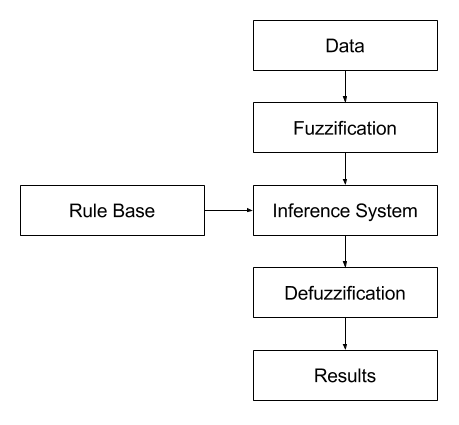
\includegraphics[scale=0.6]{fig1}
\caption{Fuzzy Logic System}
\end{figure}

% needed in second column of first page if using \IEEEpubid
%\IEEEpubidadjcol

% An example of a floating figure using the graphicx package.
% Note that \label must occur AFTER (or within) \caption.
% For figures, \caption should occur after the \includegraphics.
% Note that IEEEtran v1.7 and later has special internal code that
% is designed to preserve the operation of \label within \caption
% even when the captionsoff option is in effect. However, because
% of issues like this, it may be the safest practice to put all your
% \label just after \caption rather than within \caption{}.
%
% Reminder: the "draftcls" or "draftclsnofoot", not "draft", class
% option should be used if it is desired that the figures are to be
% displayed while in draft mode.
%
%\begin{figure}[!t]
%\centering
%\includegraphics[width=2.5in]{myfigure}
% where an .eps filename suffix will be assumed under latex, 
% and a .pdf suffix will be assumed for pdflatex; or what has been declared
% via \DeclareGraphicsExtensions.
%\caption{Simulation Results}
%\label{fig_sim}
%\end{figure}

% Note that IEEE typically puts floats only at the top, even when this
% results in a large percentage of a column being occupied by floats.


% An example of a double column floating figure using two subfigures.
% (The subfig.sty package must be loaded for this to work.)
% The subfigure \label commands are set within each subfloat command, the
% \label for the overall figure must come after \caption.
% \hfil must be used as a separator to get equal spacing.
% The subfigure.sty package works much the same way, except \subfigure is
% used instead of \subfloat.
%
%\begin{figure*}[!t]
%\centerline{\subfloat[Case I]\includegraphics[width=2.5in]{subfigcase1}%
%\label{fig_first_case}}
%\hfil
%\subfloat[Case II]{\includegraphics[width=2.5in]{subfigcase2}%
%\label{fig_second_case}}}
%\caption{Simulation results}
%\label{fig_sim}
%\end{figure*}
%
% Note that often IEEE papers with subfigures do not employ subfigure
% captions (using the optional argument to \subfloat), but instead will
% reference/describe all of them (a), (b), etc., within the main caption.


% An example of a floating table. Note that, for IEEE style tables, the 
% \caption command should come BEFORE the table. Table text will default to
% \footnotesize as IEEE normally uses this smaller font for tables.
% The \label must come after \caption as always.
%
%\begin{table}[!t]
%% increase table row spacing, adjust to taste
%\renewcommand{\arraystretch}{1.3}
% if using array.sty, it might be a good idea to tweak the value of
% \extrarowheight as needed to properly center the text within the cells
%\caption{An Example of a Table}
%\label{table_example}
%\centering
%% Some packages, such as MDW tools, offer better commands for making tables
%% than the plain LaTeX2e tabular which is used here.
%\begin{tabular}{|c||c|}
%\hline
%One & Two\\
%\hline
%Three & Four\\
%\hline
%\end{tabular}
%\end{table}


% Note that IEEE does not put floats in the very first column - or typically
% anywhere on the first page for that matter. Also, in-text middle ("here")
% positioning is not used. Most IEEE journals use top floats exclusively.
% Note that, LaTeX2e, unlike IEEE journals, places footnotes above bottom
% floats. This can be corrected via the \fnbelowfloat command of the
% stfloats package.



\section{Working Principle}

\subsection{Data Collection}

A college student is carrying his/her smart phone everywhere. Hence using the GPS we can extract his/her position throughout the day. In the application and testing of this paper, the mobile application was developed on Android while the point of interest was extracted using Google Maps API by querying the user\rq s location extracted from GPS. Google Maps API classifies most of the locations into various categories namely \texttt{restaurant}, \texttt{shopping\_mall}, \texttt{city\_hall} etc. Let us refer to all these categories hence forward as \textit{tags}. Apart from these existing tags, we generate two additional tags namely \texttt{home} and \texttt{work}. The GPS data for these two additional tags would be user specific. Hence initially every user needs to update their location for these two tags specifically. This step is conducted so as to recognize distinctly one\rq s home and workplace which in further course would generate accurate results. Let consider this example, one might go to a pizza shop to hang out with friends and family. However if someone is working in a pizza shop and the GPS details of the specific pizza shop is not known beforehand, it is very likely that one might consider this entire working time as time utilized for hanging out with friends. However if the person goes to some other pizza shop it is very likely he is going out with friends. To avoid this confusion this initial step has to be carried out.

Let $\mathbf{X}$ be the set of all tags defined as $\mathbf{X} = \{x \mid x\text{ is a tag}\}$. Analysing the way a person lives is governed by many parameters, but in a typical student\rq s life we are mainly concerned about one\rq s health, education, leisure and social life. However a person also invests certain amount of time which fails to fall under these categories. A example of this would be travelling time. Activities like these fall under the \textit{other} category. Now let $S$, $L$, $H$, $W$, $O$ be subsets of $\mathbf{X}$ defined as
\begin{align*}
S =\ &\{x \mid x \in \mathbf{X},\ x = \text{social}\ \textrm{and}\ x \neq \text{home, work}\} \\
L =\ &\{x \mid x \in \mathbf{X},\ x = \text{leisure}\ \textrm{and}\ x \neq \text{home, work}\} \\
H =\ &\{x \mid x \in \mathbf{X},\ x = \text{health}\ \textrm{and}\ x \neq \text{home, work}\} \\
W =\ &\{x \mid x \in \mathbf{X},\ x = \text{work}\ \textrm{and}\ x \neq \text{home}\} \\
O =\ & \{x \mid x \in \mathbf{X}\ \textrm{and}\ x \notin S\cup L\cup H\cup W \}
\end{align*}
A \textit{tag} $x$ might belong to one or more of the sets $S,\ L,\ H,\ W$. For example, a person might visit an Amusement Park. In this case the person\rq s \textit{social} and \textit{leisure} scores are both incremented. Using this categorization technique we can extract one\rq s location and time spent at each \textit{tag} for the entire day. TABLE I lists down some locations and their possible purpose of visits. The locations mentioned are basically \textit{tags} other than \texttt{home} and \texttt{work}.
\begin{table}
\small
\captionof{table}{Sample locations and purposes}
\begin{center}
\def\arraystretch{1.7}
\begin{tabular}{|l|l|}
\hline
 \bf Location & \bf Purpose \\
 \hline
 Cafe, Restaurant & Going out with friends and family. \\
 \hline
 Supermarket, Gas Station & Chores \\
 \hline
 Gym, Ground, Hospital & Exercise or Health Treatment \\
 \hline
 Cinema Hall, Spa & Leisure and Relaxation \\
\hline
Bank, Business Associates & Work \\
\hline
\end{tabular}
\end{center}
\end{table}

\textbf{Weighing criteria}: For a given purpose, different locations would have different amount of productivity and impact. For example, hospital and gym both fall under the \textit{health} category. However one visits a gym to increase his physical activity and hence visiting a gym has a positive impact on one\rq s health. However one visits a hospital if he/she has fallen sick. Hence, visiting a hospital has a negative impact on one\rq s health. So we have to handle these two situations differently.

We define a function $Y:\mathbf{X} \rightarrow \mathbb{R}$ such that $Y(x)$ for every $x \in \mathbf{X}$ denotes the time spent at the location \textit{tag} $x$. For example, let $x = \text{gym}$. Say $Y(x) = 0.5$. This implies a person has spent $30$ minutes at a \textit{gym} in the entire day. The unit of time is set in hours throughout this paper.

We define a function $Z_S:S \rightarrow [-100, 100]$ such that $Z_S(x)$ for every $x \in S$ denotes the intensity of the \textit{tag} $x$ with respect to the \textit{social} category. Similarly we define $Z_H$, $Z_L$, $Z_W$, and $Z_O$ for the \textit{health}, \textit{leisure}, \textit{work}, and \textit{other} categories respectively. The range $[-100, 100]$ is chosen for normalization purposes. For example, let $x = \text{gym}$. Say $Z_H(x) = 50 > 0$ as gym has a positive health impact. Let $y = \text{hospital}$, then $Z_H(y) = -20 < 0$ as hospital has a negative health impact. However, $Z_L(x) = Z_L(y) = 0$ as both $x$ and $y$ don\rq t contribute to the \textit{leisure} category. Also note that if a \textit{tag} $t$ belongs to two different categories, then its weightage in both the categories cannot be $0$.

For both $Y$ and $Z$ we have excluded the \textit{home} tag as it is a special case. This is explained later.

\begin{figure}[h!]
\centering
\captionsetup{justification=centering}
\noindent 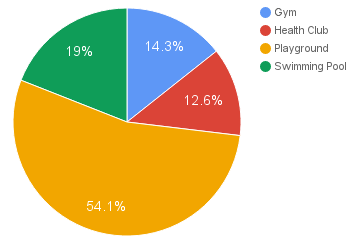
\includegraphics[scale=0.6]{fig2}
\caption{Survey for \textit{positive} health weights}
\end{figure}
\begin{figure}[h!]
\centering
\captionsetup{justification=centering}
\noindent 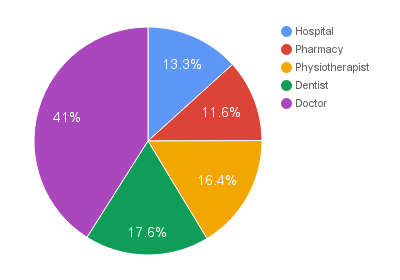
\includegraphics[scale=0.6]{fig3}
\caption{Survey for \textit{negative} health weights}
\end{figure}
\textbf{Assigning weights}: One is free to assign the weights independently. However for better results, we assign weights by conducting a survey to understand how appropriately a location \textit{tag} fulfils the purpose of a category. For instance consider the \textit{health} category. In the survey we ask a sample population to rank every $x \in H$ in an order of fulfilment of their positive \textit{health} benefits. Consider the following survey with 
\begin{align*}
H =\ \{&\text{gym},\ \text{playground},\ \text{swimming\_pool}, \text{health\_club},\\
&\text{hospital},\ \text{pharmacy},\ \text{physiotherapist},\ \text{dentist},\ \text{doctor}\}
\end{align*}

Fig. 2 shows a survey for determining \textit{positive} weights in the \textit{health} category. As $54.1\%$ people taking the survey voted \textit{playground} as their maximum positive benefit from the \textit{health} category, the corresponding weight for $x = \text{playground}$ is computed as $Z_H(x) = \frac{54.1}{100} \times 100 = 54.1$.

Fig. 3 shows a survey for determining \textit{negative} weights in the \textit{health} category. As $41\%$ people taking the survey voted \textit{doctor} as their maximum non fulfilment from the \textit{health} category, the corresponding weight for $x = \text{doctor}$ is computed as $Z_H(x) = -\frac{41}{100} \times 100 = -41$.

\textbf{Home tag}: The time spent at the \textit{home} location might not be entirely used for rest and leisure purpose only. One might practice yoga at one\rq s home and the equivalent time should be added to the \textit{health} category. Let $\tau$ denote the total time spent at \textit{home}. And $\tau_H$, $\tau_W$, $\tau_L$, $\tau_O$, $\tau_S$ denote the equivalent time in respective categories. This time is taken as user input through the mobile application. For better results a random push notification system can be used to learn the characteristics of the user. The home tag will be associated with weights $\xi_H$, $\xi_S$, $\xi_L$, $\xi_W$, $\xi_O$ which denote the intensity of the tags at \textit{home}. For instance, $\xi_W=30$ and $Z_W(\text{office}) = 50 > 30$ as working at \textit{home} might not be as productive as working at \textit{office}.

\subsection{Fuzzification}

\textbf{Fuzzification of time}: Consider a person $p$. Suppose $p$ visits tags $\{x_1, x_2, \ldots, x_n\}$, with the time spent at these locations denoted by $\{Y(x_1), Y(x_2), \ldots, Y(x_n)\}$. Let $K_H$, $K_L$, $K_S$, $K_W$, $K_O$ denote the overall time spent in \textit{health}, \textit{leisure}, \textit{social}, \textit{work}, and \textit{other} categories respectively. Then 
\[
K_H = \sum_{x_i \in H}Y(x_i) + \tau_H
\]
Similarly, $K_W$, $K_S$, $K_L$, $K_O$ are defined.

We define the following fuzzy sets for all the categories. These sets define the type of lifestyle a person is living in each category. Here \textit{leisure} also includes rest.
\begin{align*}
\textit{health}=&\ \{\text{unfit},\ \text{fit},\ \text{proactive}\}\\
\textit{leisure}=&\ \{\text{hectic},\ \text{ideal},\ \text{lazy}\}\\
\textit{social}=&\ \{\text{reserved},\ \text{sociable},\ \text{over\_social}\}\\
\textit{work}=&\ \{\text{lethargic},\ \text{hard\_working},\ \text{industrious}\}\\
\textit{others}=&\ \{\text{non\_productive},\ \text{productive}\}
\end{align*}
The membership functions for these fuzzy sets are constructed by conducting a survey on a sample population. We will approximate the data from the survey using quantile range and trapezoidal membership functions. However, one can use various other techniques to plot membership functions. For instance, in a sample survey the hours spent by fit students in the \textit{health} category were: $0.45,\ 1.25,\ 2,\ 2.25,\ 2.5,\ 2.5,\ 2.75,\ 2.75,\ 3,\ 4,\ 4.25$. So with respect to the inter quantile range $Q_1 = 2$, $Q_2 = 2.5$, $Q_3 = 3$, $\inf = 0.45$, and $\sup = 4.25$. The trapezoidal membership function for the linguistic term "fit" under the \textit{health} category using these values is shown in Fig. $4$.

Figure $5$, $6$, $7$, $8$, and $9$ show the membership functions for each linguistic term under each category.

\begin{figure}[h!]
\centering
\captionsetup{justification=centering}
\noindent 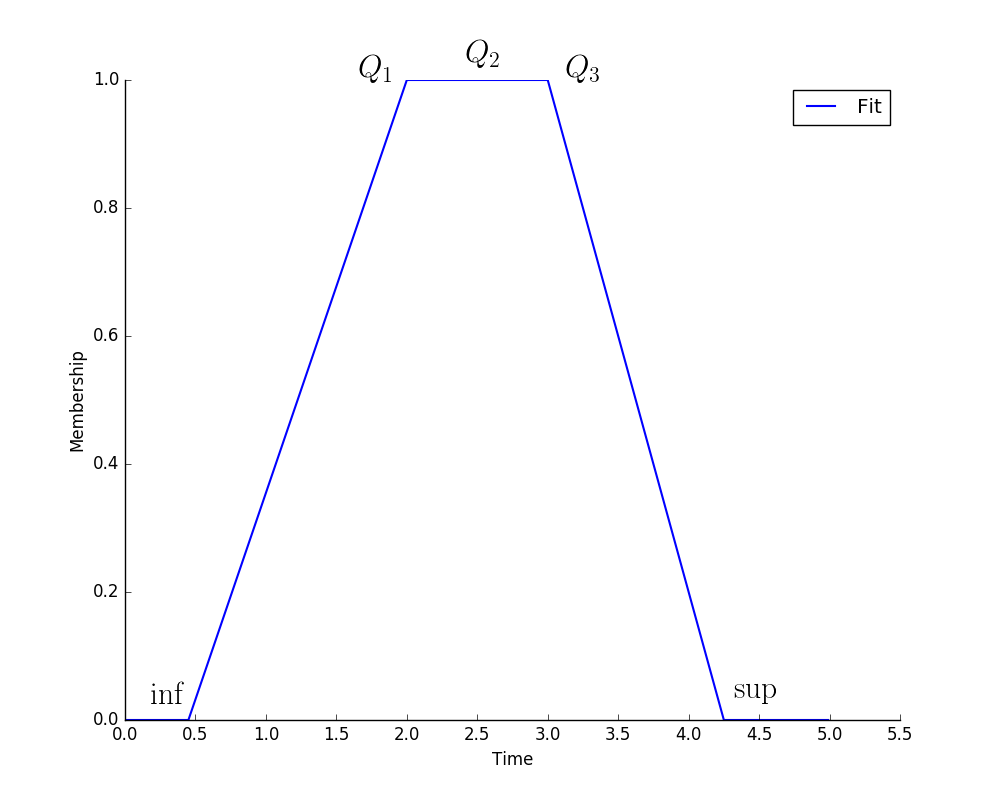
\includegraphics[scale=0.35]{fit}
\caption{Membership function for the linguistic term \textit{fit}}
\end{figure}
\begin{figure}[h!]
\centering
\captionsetup{justification=centering}
\noindent 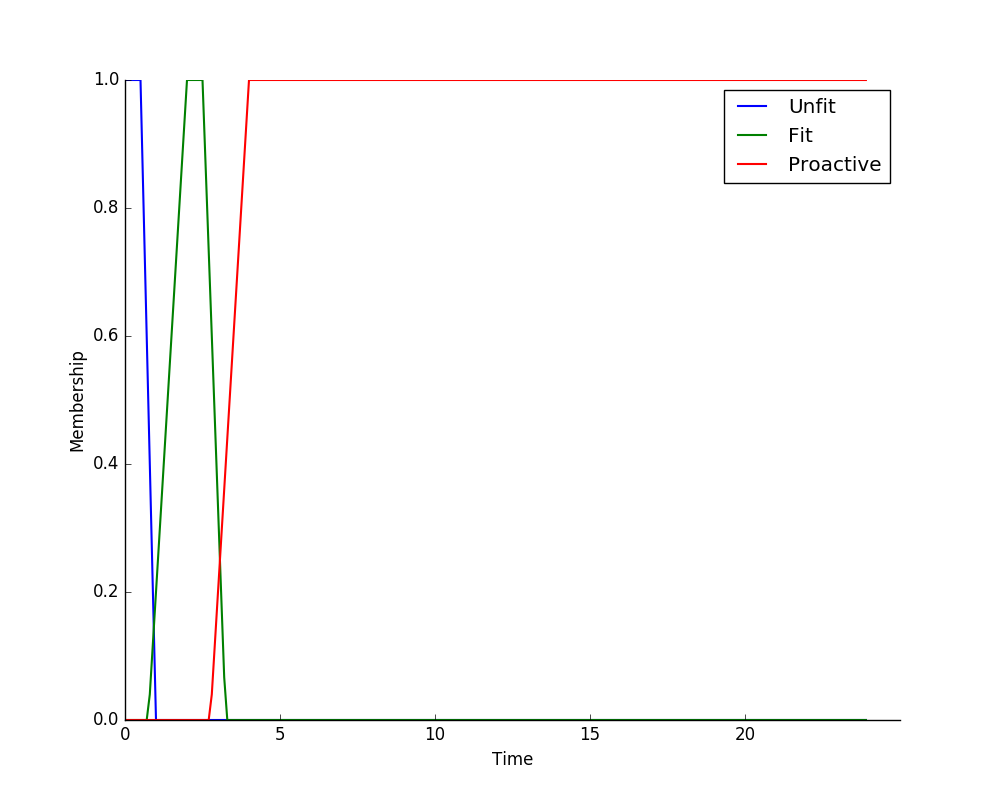
\includegraphics[scale=0.35]{health}
\caption{Membership function for \textit{health} category}
\end{figure}
\begin{figure}[h!]
\centering
\captionsetup{justification=centering}
\noindent 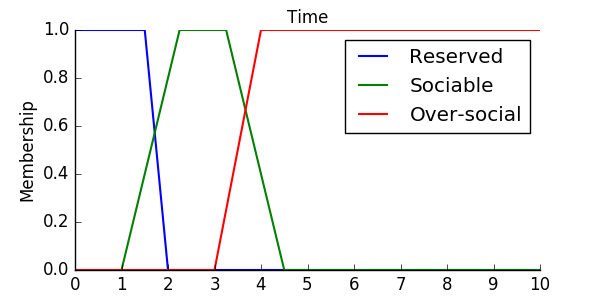
\includegraphics[scale=0.35]{social}
\caption{Membership function for \textit{social} category}
\end{figure}
\begin{figure}[h!]
\centering
\captionsetup{justification=centering}
\noindent 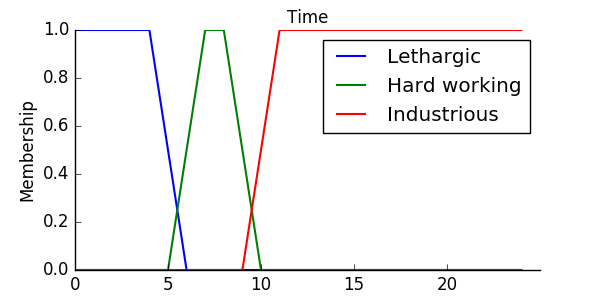
\includegraphics[scale=0.35]{work}
\caption{Membership function for \textit{work} category}
\end{figure}
\begin{figure}[h!]
\centering
\captionsetup{justification=centering}
\noindent 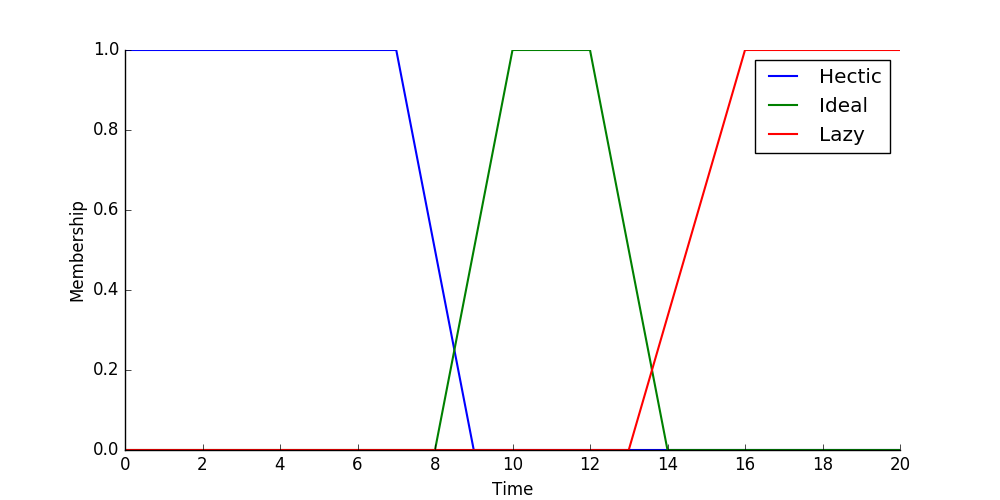
\includegraphics[scale=0.35]{leisure}
\caption{Membership function for \textit{leisure} category}
\end{figure}
\begin{figure}[h!]
\centering
\captionsetup{justification=centering}
\noindent 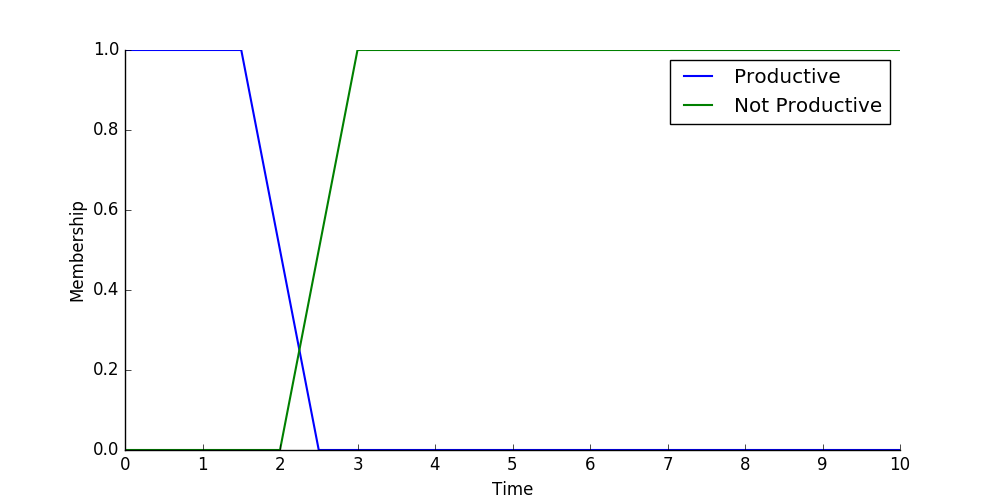
\includegraphics[scale=0.35]{other}
\caption{Membership function for \textit{other} category}
\end{figure}
\textbf{Fuzzification of score}: Not only the time spent at a location is important but also how the time is spent is important too. This effective utilisation of time is denoted by a \textit{score} $M_S$, $M_L$, $M_O$, $M_W$, and $M_H$ for the respective categories. The score for the \textit{social} category is calculated as follows
\[
M_S = \sum_{x \in S} Y(x)Z_S(x) + \tau_S\xi_S
\]
Similarly we define the other scores. The fuzzy set of linguistic terms "low\_score", "ideal\_score" and "high\_score" define the fuzzy scores in each category. The membership function of these sets in all categories is calculated similar to the fuzzy time membership functions by conducting a survey. For instance, a survey conducted on a sample of fit students is shown in TABLE II.
\begin{table}
\small
\captionof{table}{Survey to determine the membership function for the linguistic term "ideal\_score" under \textit{health} category}
\begin{center}
\def\arraystretch{1.7}
\begin{tabular}{| l | l | l |}
\hline
\bf Time $(t_i)$ & \bf Weight $(w_i)$ & \bf Score $(\sum_{i} w_it_i)$ \\
\hline
$0.45$ & $25$ & $0.45\times 25=11.25$ \\
\hline
$1$, $0.25$ & $10,\ 12$ & $1\times10+0.25\times 12=13$ \\
\hline
$2$ & $15$ & $2\times 15=30$ \\
\hline
$2.25$ & $18$ & $2.25\times 18=40.5$ \\
\hline
$2.5$ & $18$ & $2.5\times 18=45$ \\
\hline
$2.5$ & $20$ & $2.5\times 20=50$ \\
\hline
$2.75$ & $12$ & $2.75\times 12=33$ \\
\hline
$2,\ 0.75$ & $13,\ 10$ & $2\times 13+0.75\times 10=33.5$ \\
\hline
$3$ & $11$ & $3\times 11=33$ \\
\hline
$2,\ 2$ & $13,\ 8$ & $2\times 13+2\times 8=42$ \\
\hline
$4.25$ & $7$ & $4.25\times 7 =29.75$ \\
\hline
\end{tabular}
\end{center}
\end{table}
Hence $\inf = 11.25,\ Q_1=29.75,\ Q_3=42,\ \sup = 50$.  Accordingly the membership function for the linguistic term "ideal\_score" under the health category is shown in Fig. 10. Similarly we can plot plot the membership functions for the entire fuzzy set across all categories.
\begin{figure}[h!]
\centering
\captionsetup{justification=centering}
\noindent 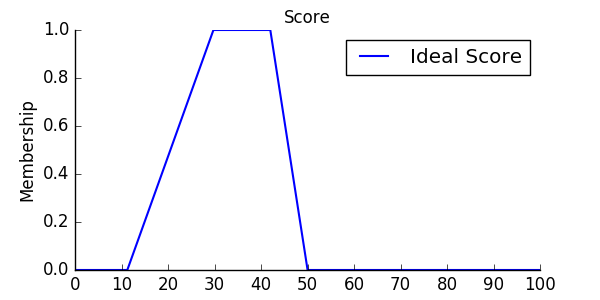
\includegraphics[scale=0.35]{ideal_health}
\caption{Membership function for "ideal\_score" under \textit{health} category}
\end{figure}
\subsection{Defuzzification}
\begin{figure}[h!]
\centering
\captionsetup{justification=centering}
\noindent 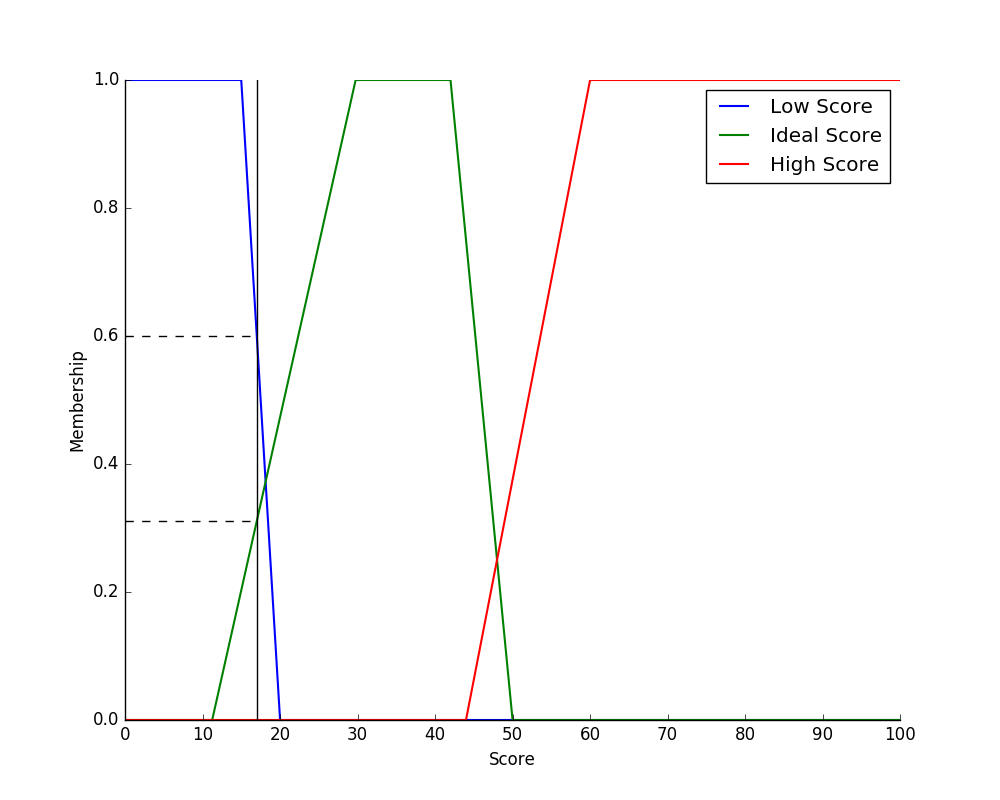
\includegraphics[scale=0.35]{health_score}
\caption{Calculation of membership values}
\end{figure}
Given the input data, $Y(x)$, $Z_i(x)$, $\tau_i$, and $\xi_i$ where $x \in \mathbf{X}$ and $i = S,\ L,\ O,\ W,\ H$, we calculate corresponding $K_i$ and $M_i$. Using surveys we determine the membership functions for all linguistic terms in all categories for both fuzzification of time and score. Then we determine the membership value of $K_i$ and $M_i$ in the respective categories for all the linguistic terms. Let $\{R_1, R_2, \ldots, R_N\}$ be a set of recommendations. Now every $R_k\ (1 \leq k \leq N)$ will be dependent on a set of linguistic terms. For example, a recommendation $R = \textit{"All work and no play makes Jack a dull boy."}$ will be outputted if a person is spending too much time and effort in work and less in his leisure and social life. That is he/she has a "industrious" work life with a high work score and has a "reserved" social life with a low social score and a "hectic" life with respect to leisure with a low score. So attributes of $R$ can be represented as $\{K_W=\text{"industrous"},\ M_W=\text{"high\_score"},\ K_S=\text{"reserved"},\ M_S=\text{"low\_score"},\ K_L=\text{"hectic"},\ M_L=\text{"low\_score"}\}$.

Let $R_k$ be a recommendation with attributes $\{a_1, a_2, a_3, \ldots, a_n\}$. Here each $a_j\ (1 \leq j \leq n)$ is a combination of score/time with respect to a linguistic term of a category. Hence as shown previously we can calculate its membership value. Let $\mu_1, \mu_2, \mu_3, \ldots, \mu_n$ denote the respective membership values for each attribute. Here $n$ can vary for each $R_k$.  For instance, Fig. 11 shows the membership functions of $M_H$. Let $a_1$, $a_2$, $a_3$ be the following attributes
\begin{align*}
a_1\ =&\ M_H:low\_score\\
a_2\ =&\ M_H:ideal\_score\\
a_3\ =&\ M_H:high\_score
\end{align*}
Hence $\mu_1$, $\mu_2$, $\mu_3$ for $M_H=17$ as seen from Fig. 11 will be $0.6$, $0.310$, $0.0$ respectively. Using equal weighing criteria for each $a_j$, we can calculate a score of each recommendation $\rho(R_k)$ defined as
$$\rho(R_k) = \frac{1}{n}\sum_{j=1}^{n} \mu_j$$
Now, using the \textit{most probable criterion} the recommendation with the maximum score value $\rho(R_k)$ will be displayed as output.

\section{Experiment}
A survey conducted in IIT Kharagpur was conducted to determine all the membership functions for all linguistic terms across all the categories. Some of the membership functions are shown in this paper. We also installed the mobile application on students' smart phones and analysed the results. We picked a random student and analysed his data for a day. TABLE III shows the \textit{tags} he visited throughout the day and their corresponding time and weights. The score for each \textit{tag} is also enumerated. TABLE IV shows the total time and score across all the categories. We considered the recommendations in the set $R$ where $R = \{R_1, R_2, R_3, R_4\}$.
\begin{align*}
R_1 =\ &\textit{"Catch up a movie this evening."}\\
R_2 =\ &\textit{"Work is worship."}\\
R_3 =\ &\textit{"Family matters."}\\
R_4 =\ &\textit{"Hit the gym."}
\end{align*}
The attributes of $R$ is shown in TABLE V. The membership values for each attribute is shown in TABLE VI and the corresponding score of each recommendation is also enumerated. As $\rho(R_1)$ is maximum the mobile application would recommend the student to \textit{"Catch up a movie this evening."}
\begin{table}
\small
\captionof{table}{Experiment: Data}
\begin{center}
\def\arraystretch{1.7}
\begin{tabular}{| l | l | l | l |}
\hline
\bf Tag & \bf Time & \bf Weight & \bf Score \\
\hline
university & $Y(x)=6$ & $Z_W(x) = 50$ & $300$ \\
\hline
library & $Y(x)=4$ & $Z_W(x) = 20$ & $80$ \\
\hline
home & $\tau_W=2$ & $\xi_W=30$ & $60$ \\
& $\tau_S=0.5$ & $\xi_S=30$ & $15$ \\
& $\tau_H=0.5$ & $\xi_H=20$ & $10$ \\
& $\tau_L=6.5$ & $\xi_S=30$ & $195$ \\
& $\tau_O=1$ & $\xi_O=10$ & $10$ \\
\hline
cafe & $Y(x)=1$ & $Z_S(x)=20$ & $20$ \\
\hline
supermarket & $Y(x)=1$ & $Z_O(x)=9$ & $9$ \\
\hline
grocery & $Y(x)=0.5$ & $Z_O(x)=10$ & $5$ \\
\hline
travel & $Y(x)=1$ & $Z_O(x)=15$ & $15$ \\
\hline
\end{tabular}
\end{center}
\end{table}
\begin{table}
\small
\captionof{table}{Experiment: Calculation of total time and score for each category}
\begin{center}
\def\arraystretch{1.7}
\begin{tabular}{| l | l |}
\hline
\bf Total time & \bf Total score \\
\hline
$K_S=1.5$ & $M_S=35$ \\
\hline
$K_L=6.5$ & $M_L=195$ \\
\hline
$K_O=3.5$ & $M_O=39$ \\
\hline
$K_W=12$ & $M_W=440$ \\
\hline
$K_H=0.5$ & $M_H=10$ \\
\hline
\end{tabular}
\end{center}
\end{table}
\begin{table}
\small
\captionof{table}{Experiment: Recommendation attributes}
\begin{center}
\def\arraystretch{1.7}
\begin{tabular}{| l | l |}
\hline
\bf Recommendation & \bf Attributes \\
\hline
$R_1$ & $\{K_L = \text{"hectic"},\ M_L = \text{"less\_score"},$\\&$\ K_W=\text{"industrious"},\ M_W=\text{"high\_score"}\}$ \\
\hline
$R_2$ & $\{K_W = \text{"lethargic"},\ M_W = \text{"less\_score"},$\\& $\ K_L=\text{"lazy"},\ M_L=\text{"high\_score"}\}$ \\
\hline
$R_3$ & $\{K_S = \text{"reserved"},\ M_S = \text{"less\_score"}\}$ \\
\hline
$R_4$ & $\{K_H = \text{"unfit"},\ M_H = \text{"less\_score"}\}$ \\
\hline
\end{tabular}
\end{center}
\end{table}
\begin{table}
\small
\captionof{table}{Experiment: Recommendation score calculation}
\begin{center}
\def\arraystretch{1.7}
\begin{tabular}{| l | l | l |}
\hline
\bf Recommendation & \bf Membership Values $(\mu_{j})$ & \bf Score $(\rho(R_k))$ \\
\hline
$R_1$ & $\{1.0,\ 0.8,\ 1.0,\ 1.0\}$ & $0.95$ \\
\hline
$R_2$ & $\{0.0,\ 0.0,\ 0.0,\ 0.0\}$ & $0.0$ \\
\hline
$R_3$ & $\{1.0,\ 0.7\}$ & $0.85$ \\
\hline
$R_4$ & $\{1.0,\ 0.8\}$ & $0.9$ \\
\hline
\end{tabular}
\end{center}
\end{table}
% if have a single appendix:
%\appendix[Proof of the Zonklar Equations]
% or
%\appendix  % for no appendix heading
% do not use \section anymore after \appendix, only \section*
% is possibly needed

% use appendices with more than one appendix
% then use \section to start each appendix
% you must declare a \section before using any
% \subsection or using \label (\appendices by itself
% starts a section numbered zero.)
%

\section{Conclusion}
Time management has always been a difficult art to master. This paper helps one master it by using fuzzy logic to understand the science behind this art. The use of this technology in the long run would lead to more accurate results. The main highlights of this method is that most of the segments are self configurable. The dynamics of a student studying in university $A$ and that of a student in university $B$ can be very different due to a lot of factors such as geographic location, nature of university and infrastructure. Hence the parameters for analysis of these two students should be significantly different. This paper gives the user this flexibility to configure various attributes such as weight of tags, type of membership functions and the set of recommendations. This practice would yield better results.
The long term applications are vast. This method can be used to access the performance of all students in an university. The results can be shared with the university so that the university can take appropriate actions for the welfare of the students in general.
% use section* for acknowledgement
\section*{Acknowledgment}
The authors would like to thank Professor Sudhir Kumar Barai of the Civil Engineering Department, IIT Kharagpur for his continued and unconditional guidance. An exemplary teacher and a magnificent person, we consider ourselves lucky to have been taught by him and to have worked under his supervision. Without his course, "Soft Computing Tools in Engineering", and his co-operation the preparation of this paper would not have been possible.


% Can use something like this to put references on a page
% by themselves when using endfloat and the captionsoff option.
\ifCLASSOPTIONcaptionsoff
  \newpage
\fi



% trigger a \newpage just before the given reference
% number - used to balance the columns on the last page
% adjust value as needed - may need to be readjusted if
% the document is modified later
%\IEEEtriggeratref{8}
% The "triggered" command can be changed if desired:
%\IEEEtriggercmd{\enlargethispage{-5in}}

% references section

% can use a bibliography generated by BibTeX as a .bbl file
% BibTeX documentation can be easily obtained at:
% http://www.ctan.org/tex-archive/biblio/bibtex/contrib/doc/
% The IEEEtran BibTeX style support page is at:
% http://www.michaelshell.org/tex/ieeetran/bibtex/
%\bibliographystyle{IEEEtran}
% argument is your BibTeX string definitions and bibliography database(s)
%\bibliography{IEEEabrv,../bib/paper}
%
% <OR> manually copy in the resultant .bbl file
% set second argument of \begin to the number of references
% (used to reserve space for the reference number labels box)
\begin{thebibliography}{1}

\bibitem{IEEEhowto:kopka}
H.~Kopka and P.~W. Daly, \emph{A Guide to \LaTeX}, 3rd~ed.\hskip 1em plus
  0.5em minus 0.4em\relax Harlow, England: Addison-Wesley, 1999.

\end{thebibliography}

% biography section
% 
% If you have an EPS/PDF photo (graphicx package needed) extra braces are
% needed around the contents of the optional argument to biography to prevent
% the LaTeX parser from getting confused when it sees the complicated
% \includegraphics command within an optional argument. (You could create
% your own custom macro containing the \includegraphics command to make things
% simpler here.)
%\begin{biography}[{\includegraphics[width=1in,height=1.25in,clip,keepaspectratio]{mshell}}]{Michael Shell}
% or if you just want to reserve a space for a photo:

% You can push biographies down or up by placing
% a \vfill before or after them. The appropriate
% use of \vfill depends on what kind of text is
% on the last page and whether or not the columns
% are being equalized.

%\vfill

% Can be used to pull up biographies so that the bottom of the last one
% is flush with the other column.
%\enlargethispage{-5in}




% that's all folks
\end{document}


